\section{Durchführung}
\label{sec:Durchführung}

\subsection{Versuche im elektrischen Feld}

Im ersten Versuchsteil (siehe Abb \ref{fig:V1}) wird für 5 verschiedene Beschleunigungsspannungen $U_\text{B}$ zwischen 180 und 500 V die Verschiebung des Leuchtflecks in Abhängigkeit der Ablenkspannung $U_\text{d}$ untersucht.
Dafür wird die Ablenkspannung so eingestellt, dass der Leuchtfleck nacheinander auf den 9 äquidistanten Linien des Koordinatennetzes liegt.
\begin{figure}
  \centering
  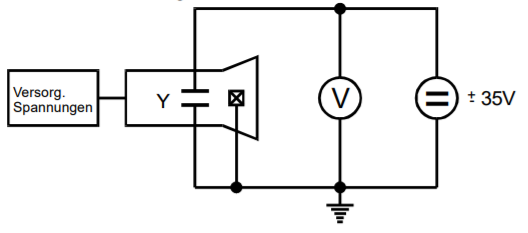
\includegraphics{data/V1.png}
  \caption{Schaltung für Ablenkung im elektischen Feld.}
  \label{fig:V1}
\end{figure}

Im zweiten Versuchsteil wird ein Oszillograph nach Abbildung \ref{fig:V2} aufgebaut.
\begin{figure}
  \centering
  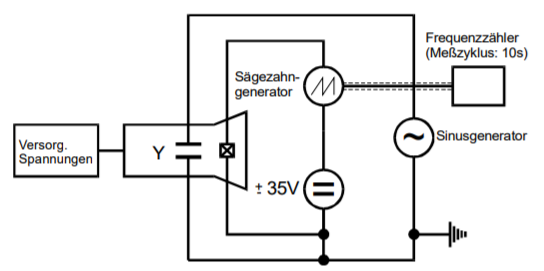
\includegraphics{data/V2.png}
  \caption{Schaltung für Oszillographen.}
  \label{fig:V2}
\end{figure}
Die Freqeunz einer Sinusspannung soll über Regulation der Sägezahnfrequenz bestimmt werden, die wie in Kapitel \ref{sec:Oszillograph} im rationalen Verhältnis zur Sinusfrequenz steht, wenn das Bild der Sinusspannung auf dem Bildschirm steht.
Außerdem soll die Amplitude der Sinusspannung über die maximale Strahlauslenkung bestimmt werden.
Für diese Berechnung muss die Beschleunigungsspannung bekannt sein.

\subsection{Versuch im magnetischen Feld}

Die spezifische Ladung der Elektronen wir mit Hilfe eines Elektronenstrahls gemessen, der durch das nahezu homogene Feld einer Helmholtz-Spule auf eine Kreisbahn abgelenkt wird.
Die Kathodenstrahlröhre wird unter Verwendung eines Deklinatorium-Inklinatorium parallel zur Horizontalkomponente des Magnetfelds ausgerichtet.
Für eine konstante Beschleunigungsspannung von 250 und 500 V wird die Abhängigkeit von $B$, das über die Spannung an den Spulen reguleirt wird und $D$, das an den Linien des Leuchtschirms abgelesen wird, untersucht.

In Nord-Süd-Richtung wirkt auf den Elektronenstrahl keine Kraft, die vom Erdmagnetfeld ausgeht, im Gegensatz zur Ost-West-Richtung.
Das Magnetfeld der Helmholtz wird so eingestellt, dass sich beide Magnetfelder gegenseitig aufheben.
Daraus kann die Größe der Horizontalkomponente des ErdMagnetfelds geschlossen werden.
Um die Totalintensität des Erdmagnetfeldes $B_\text{total}$ zu bestimmen, wird mit Hilfe des Inklinatoriums der Winkel zwischen Horizontalebene und Richtung des Erdmagnetfeldes (Inklinationswinkel) bestimmt.
